\documentclass[12pt]{article}

\usepackage[a4paper, margin=1in]{geometry}

\usepackage{listings}
\usepackage{color}
\usepackage{float}
\usepackage{graphicx}
\usepackage{subcaption}

\definecolor{codegreen}{rgb}{0,0.6,0}
\definecolor{codegray}{rgb}{0.5,0.5,0.5}
\definecolor{codepurple}{rgb}{0.58,0,0.82}
\definecolor{backcolour}{rgb}{0.95,0.95,0.92}

\lstdefinestyle{mystyle}{
  backgroundcolor=\color{backcolour},
  commentstyle=\color{codegreen},
  keywordstyle=\color{magenta},
  numberstyle=\tiny\color{codegray},
  stringstyle=\color{codepurple},
  basicstyle=\ttfamily,
  breakatwhitespace=false,
  breaklines=true,
  captionpos=b,
  keepspaces=true,
  numbers=left,
  numbersep=5pt,
  showspaces=false,
  showstringspaces=false,
  showtabs=false,
  tabsize=2
}

\lstset{style=mystyle}

\setlength\parindent{0pt}
\setlength\parskip{1em}

\title{Lab 6 - Map}
\author{\textsc{Nguyen} Duc Tung}
\date{}

\begin{document}

\maketitle

\subsection*{1. Binarization}

I get the binarization threshold from the command line, and process each pixel based on the threshold. The calculation is optimized a bit for GPU threads by using a single instruction:

\begin{lstlisting}[language=C]
binary = min(greyscale / threshold, 1) * 255;
\end{lstlisting}

\begin{figure}[H]
  \centering
  \begin{subfigure}{.45\textwidth}
    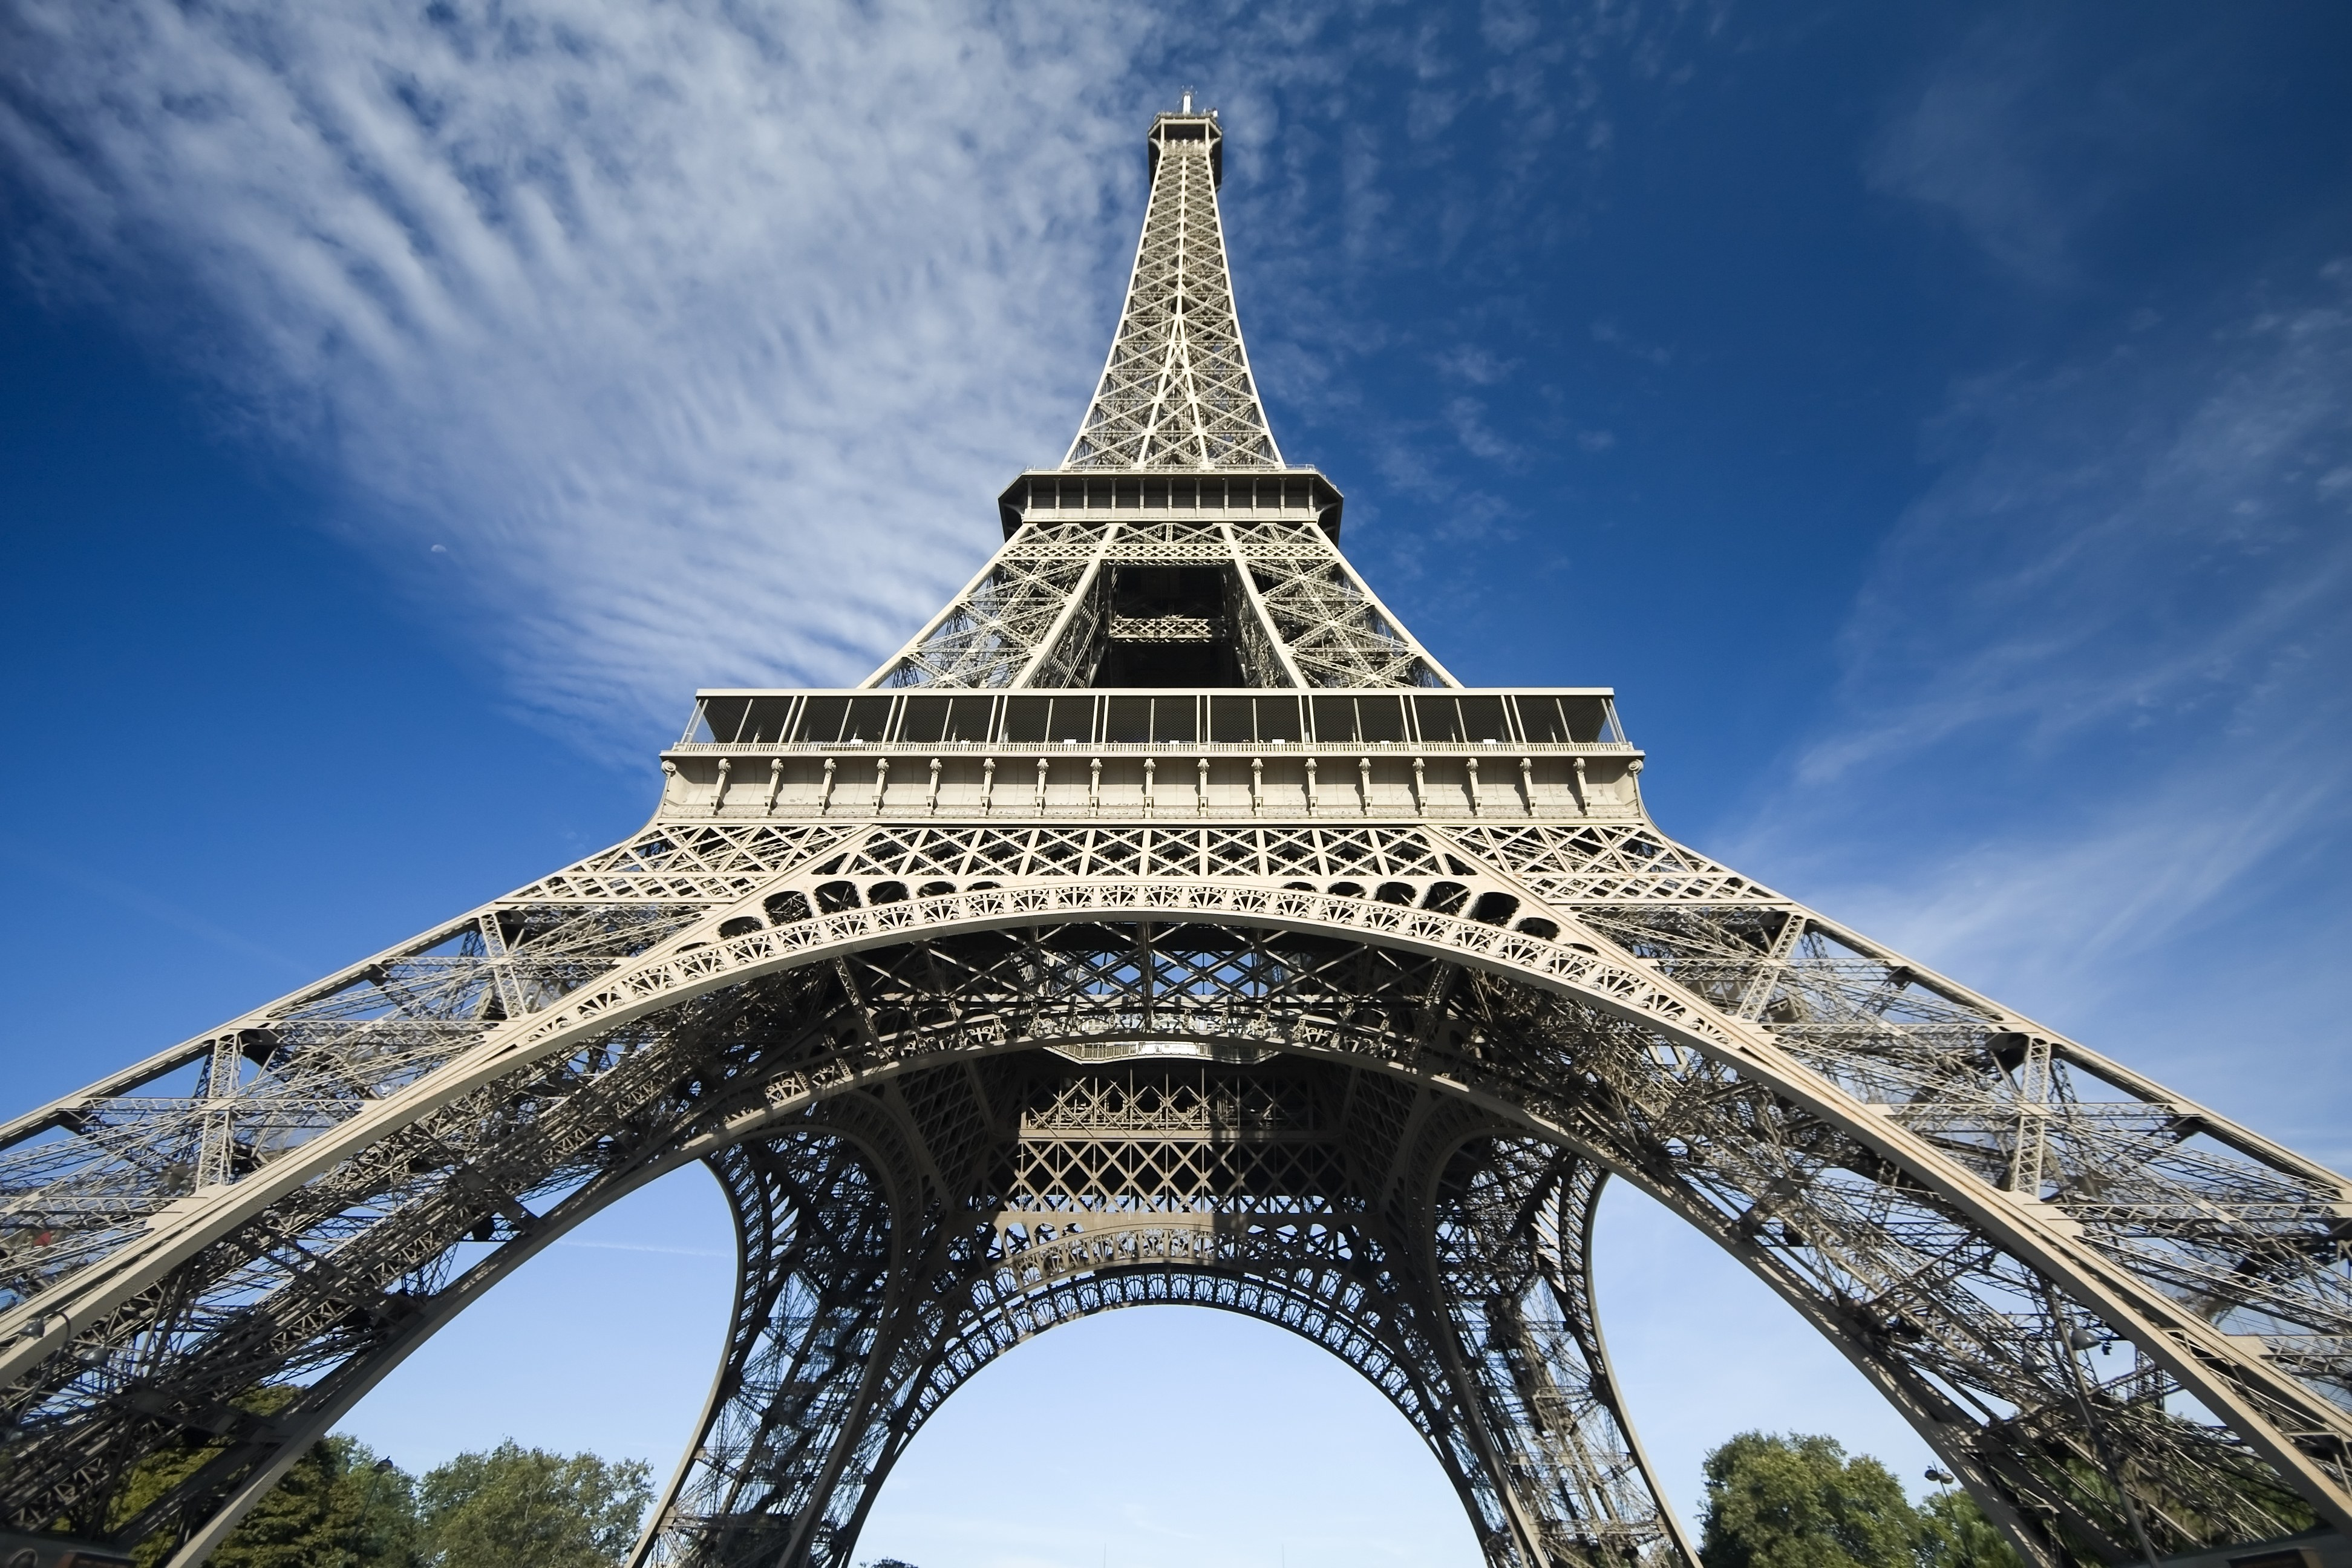
\includegraphics[width=\linewidth]{./img/origin.jpg}
    \caption{Original image}
  \end{subfigure}
  \hspace{1cm}
  \begin{subfigure}{.45\textwidth}
    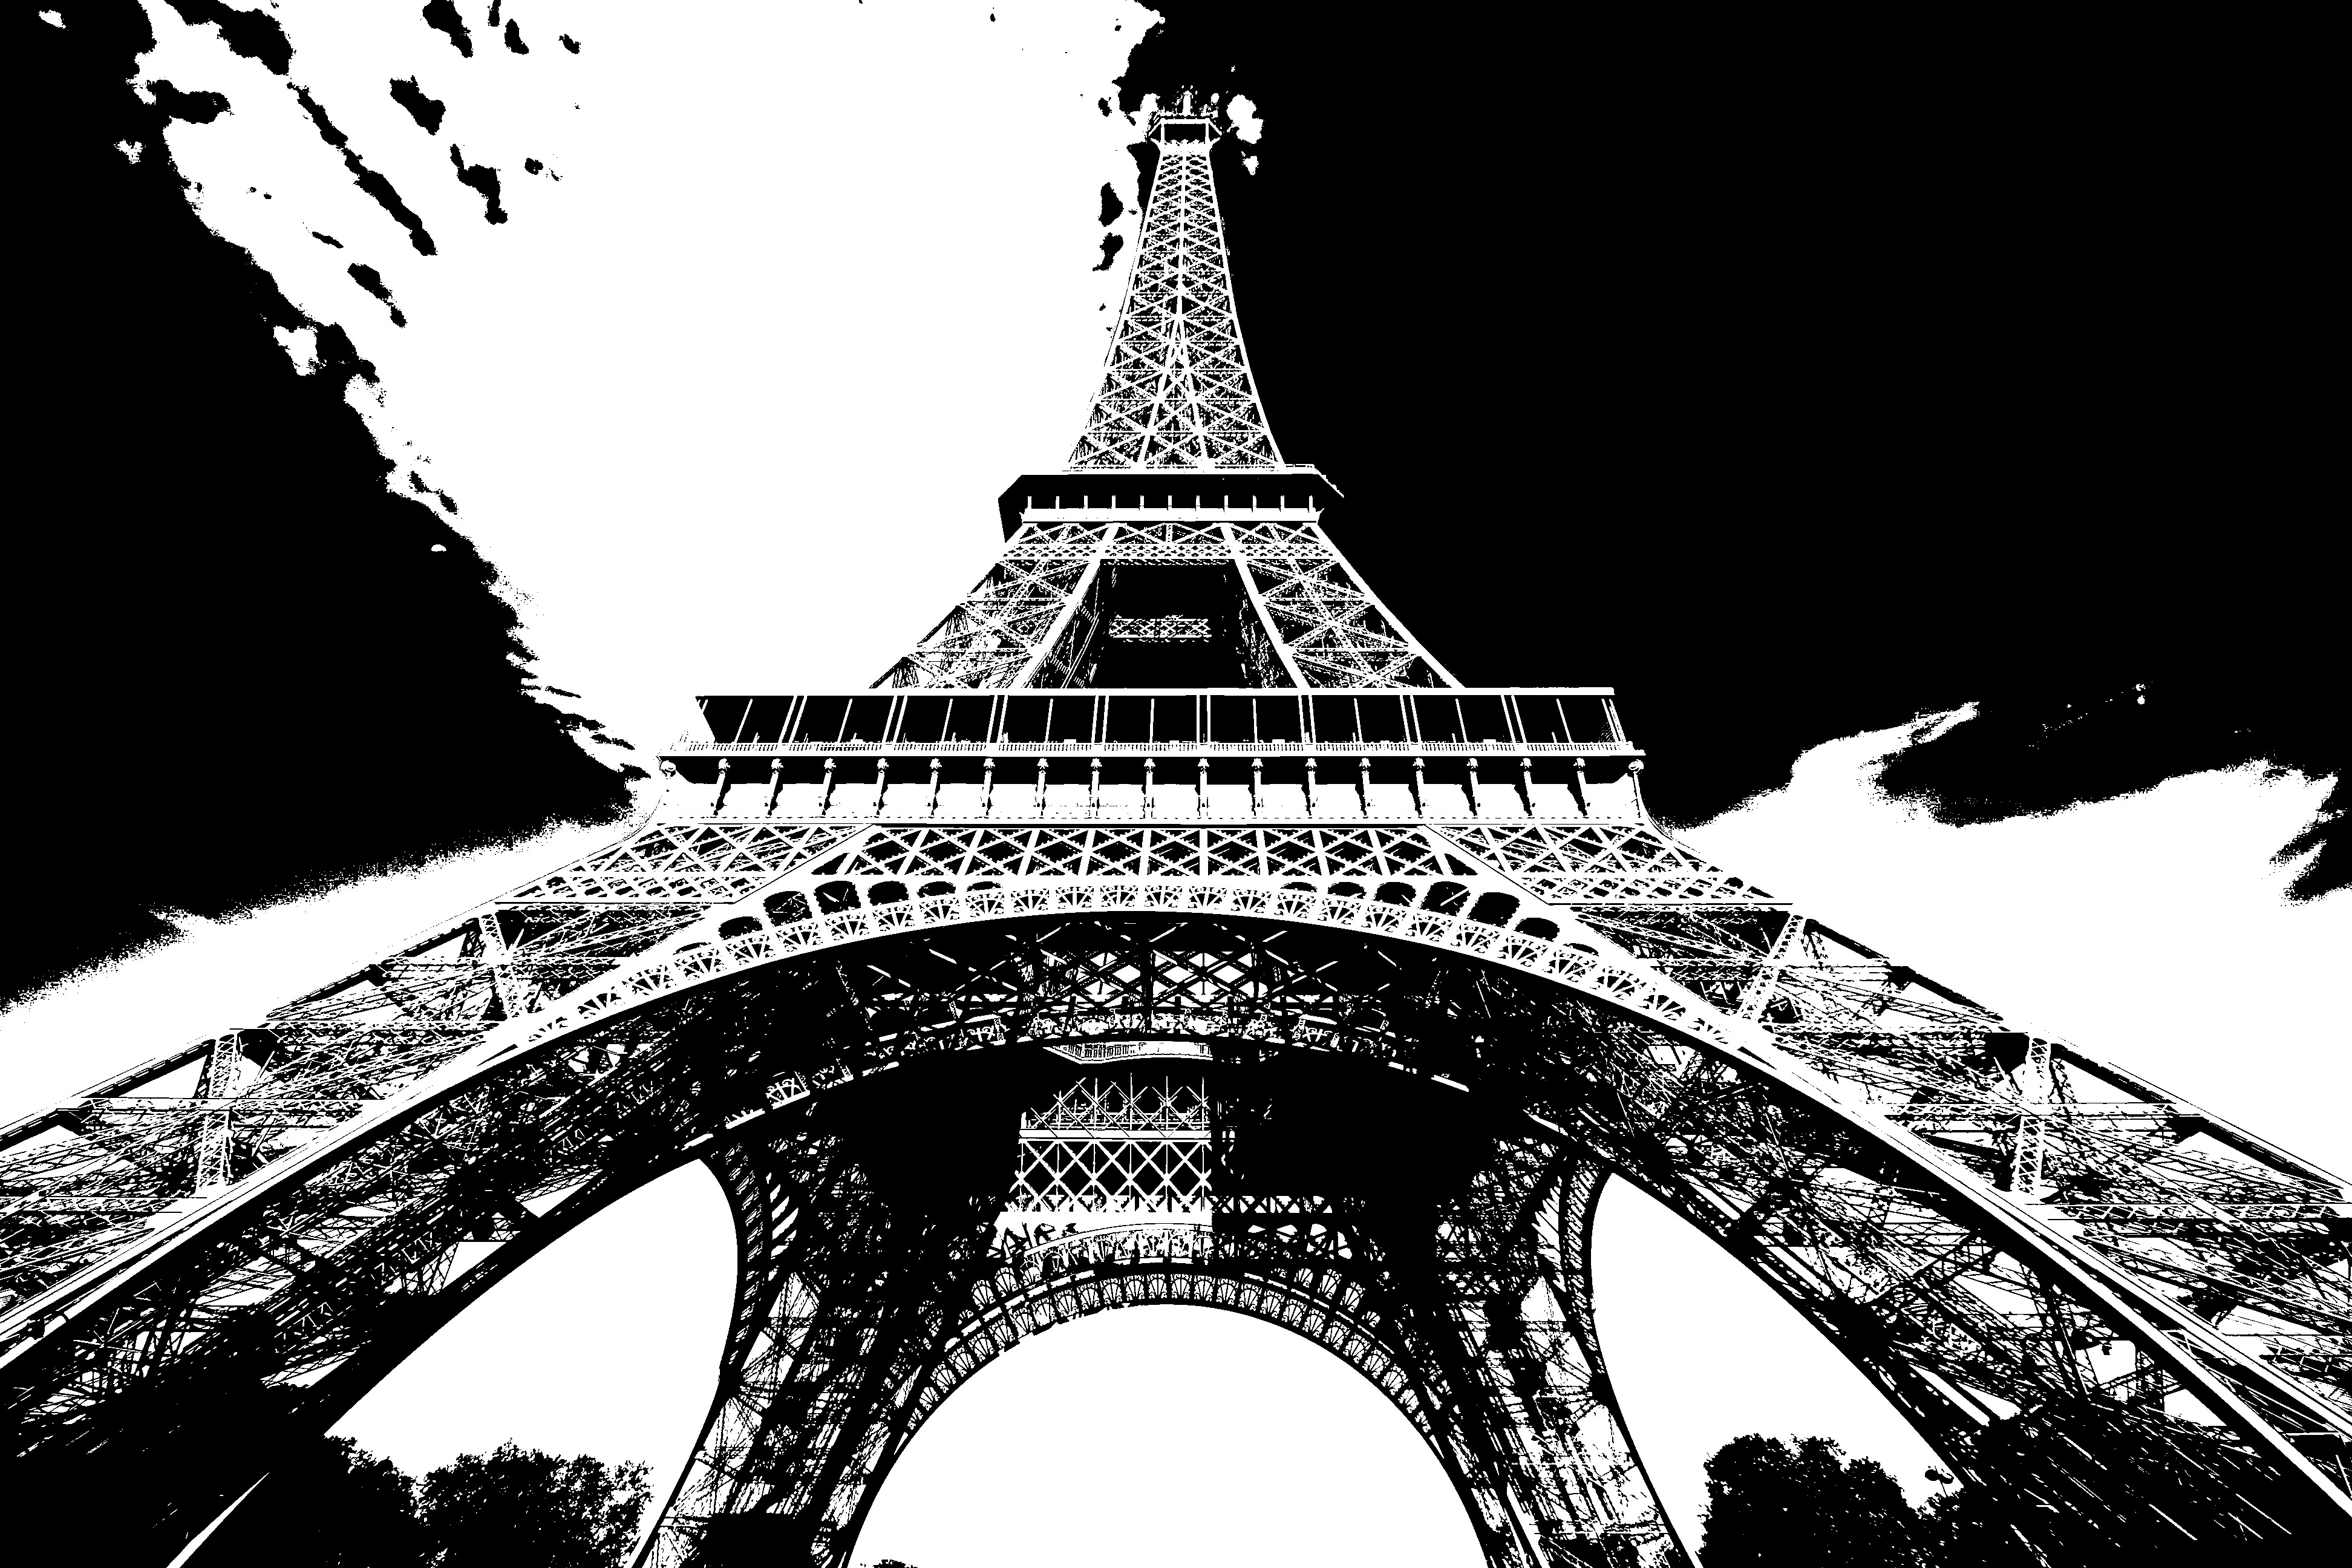
\includegraphics[width=\linewidth]{./img/6a.jpg}
    \caption{Binarization with threshold = 128}
  \end{subfigure}
\end{figure}

\subsection*{2. Brightness control}

The brightness task also get user's parameter for brightness changes. The 1-line max/min methods used to handle changes that exceed the range of color's value.

\begin{lstlisting}[language=C]
unsigned char r = min(max(input[globalId * 3] + brightnessChange, 0), 255);
unsigned char g = min(max(input[globalId * 3 + 1] + brightnessChange, 0), 255);
unsigned char b = min(max(input[globalId * 3 + 2] + brightnessChange, 0), 255);
\end{lstlisting}

\begin{figure}[H]
  \centering
  \begin{subfigure}{.45\textwidth}
    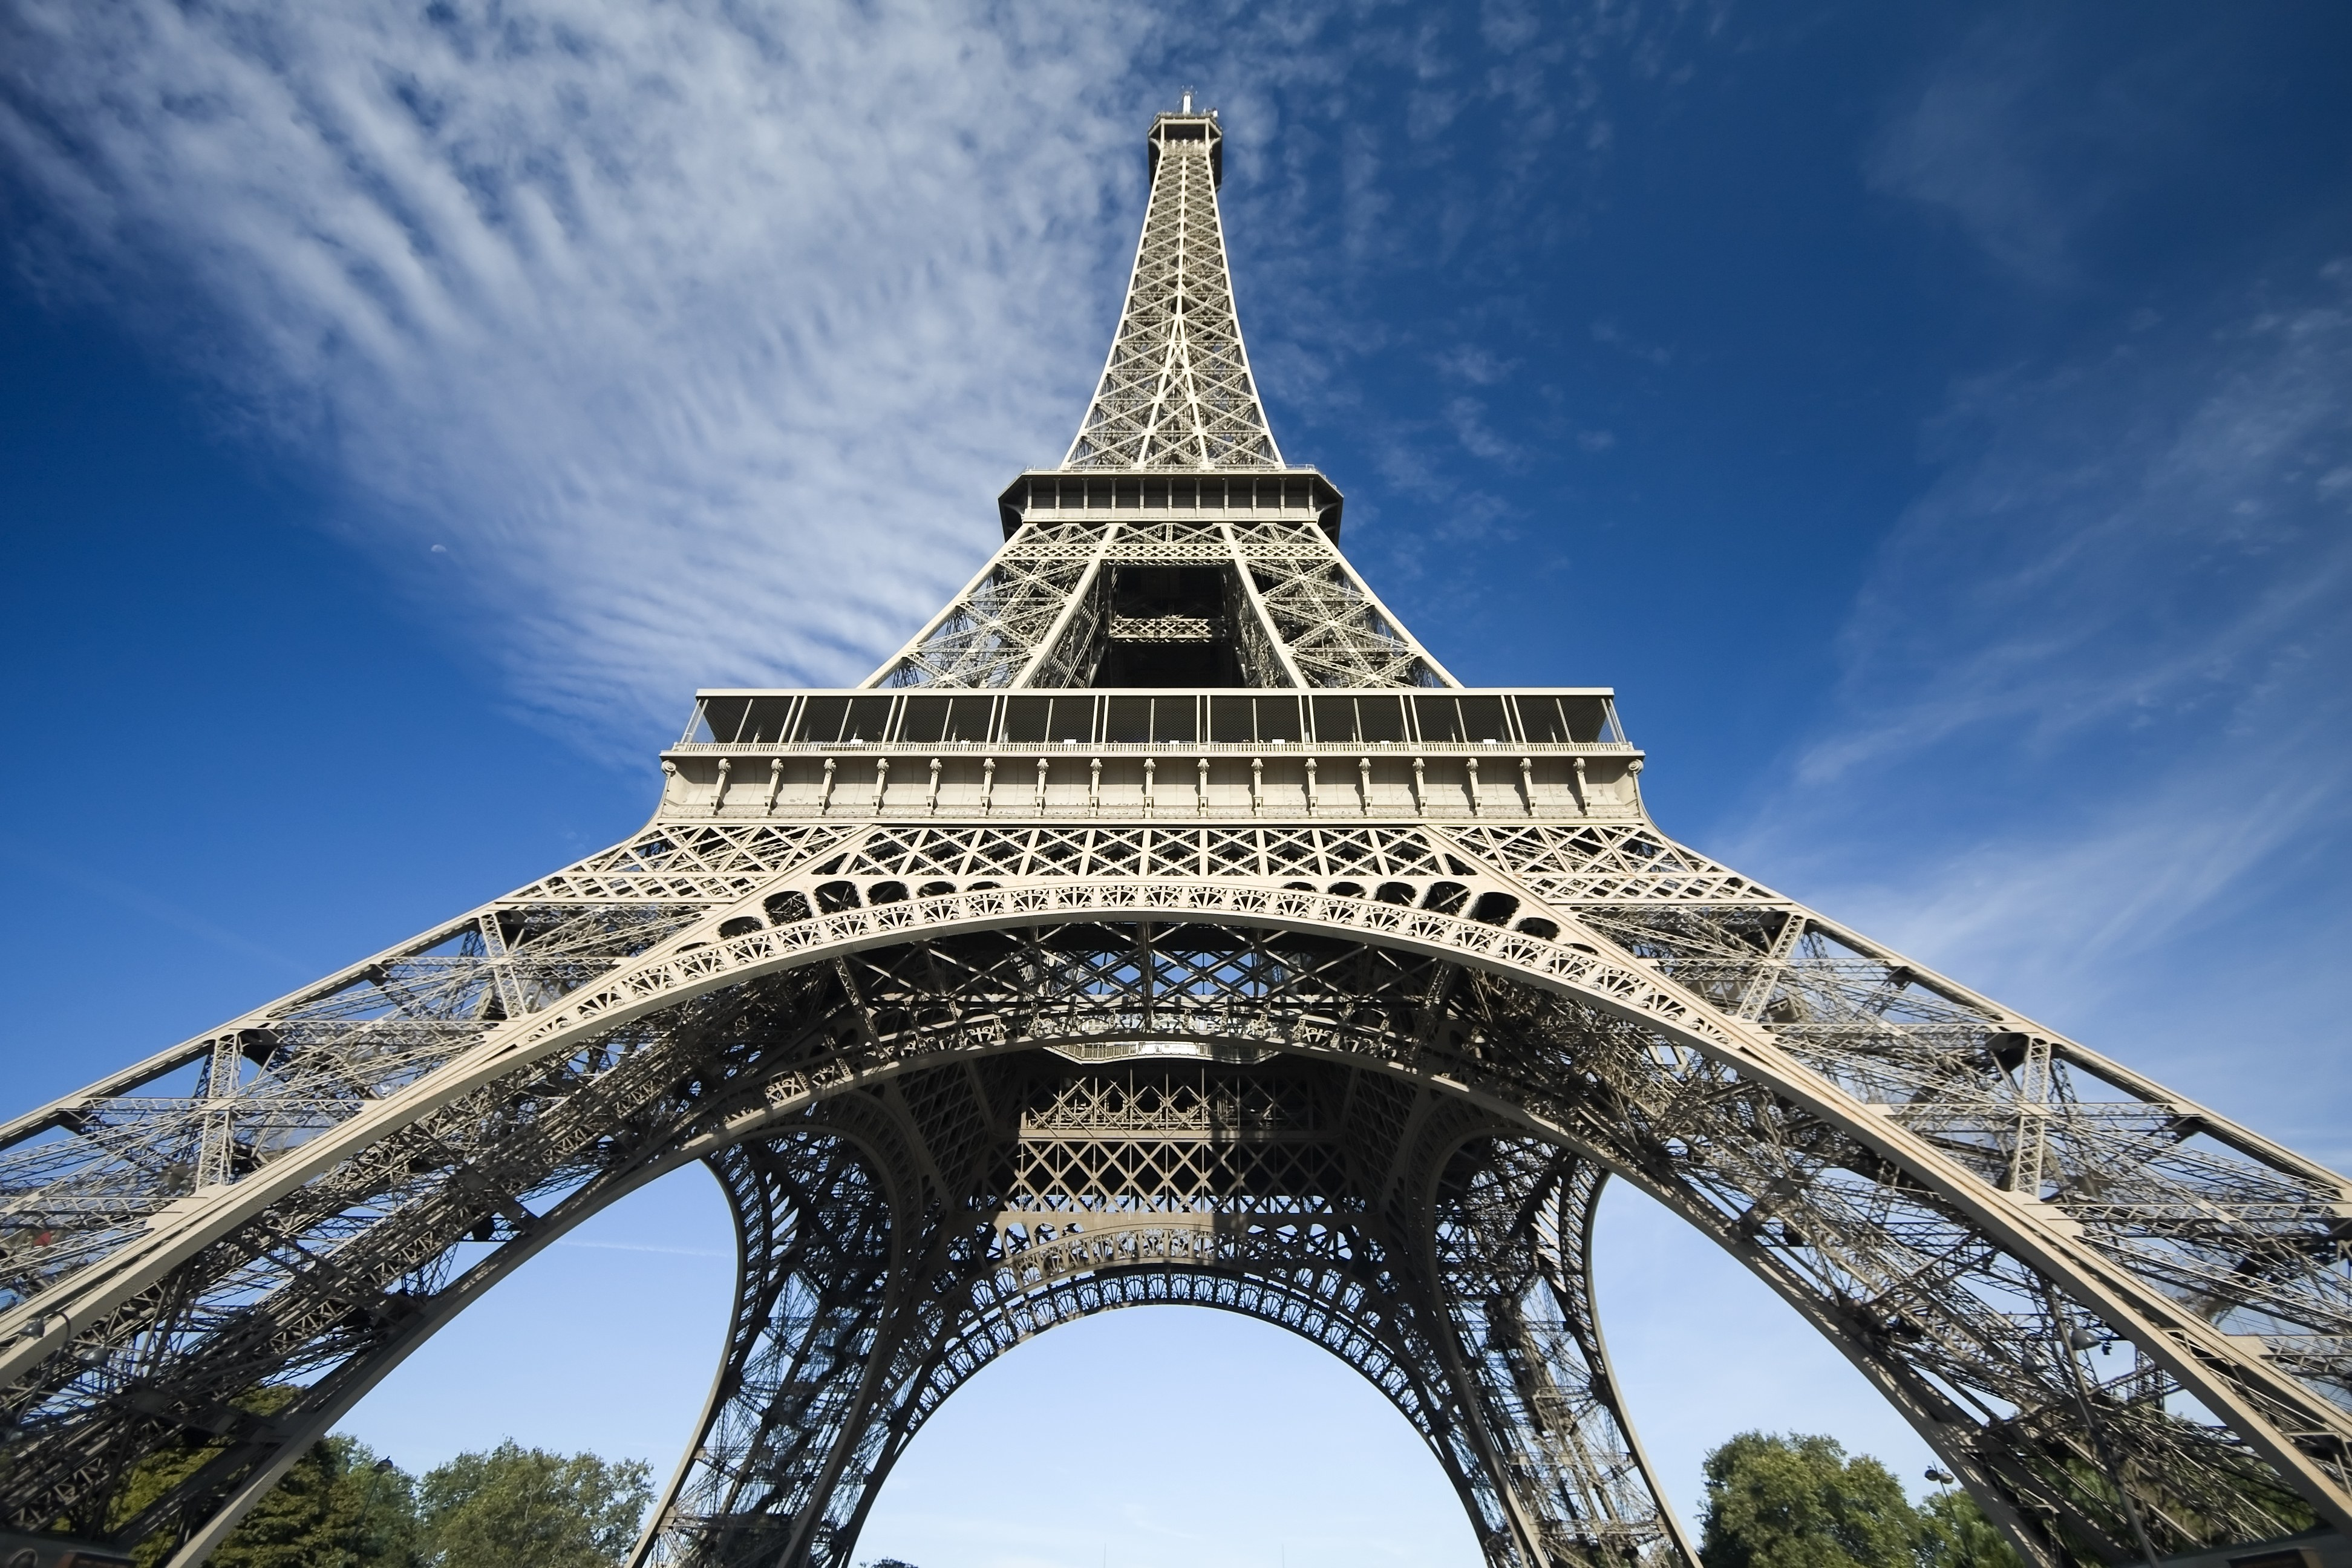
\includegraphics[width=\linewidth]{./img/origin.jpg}
    \caption{Original image}
  \end{subfigure}
  \hspace{1cm}
  \begin{subfigure}{.45\textwidth}
    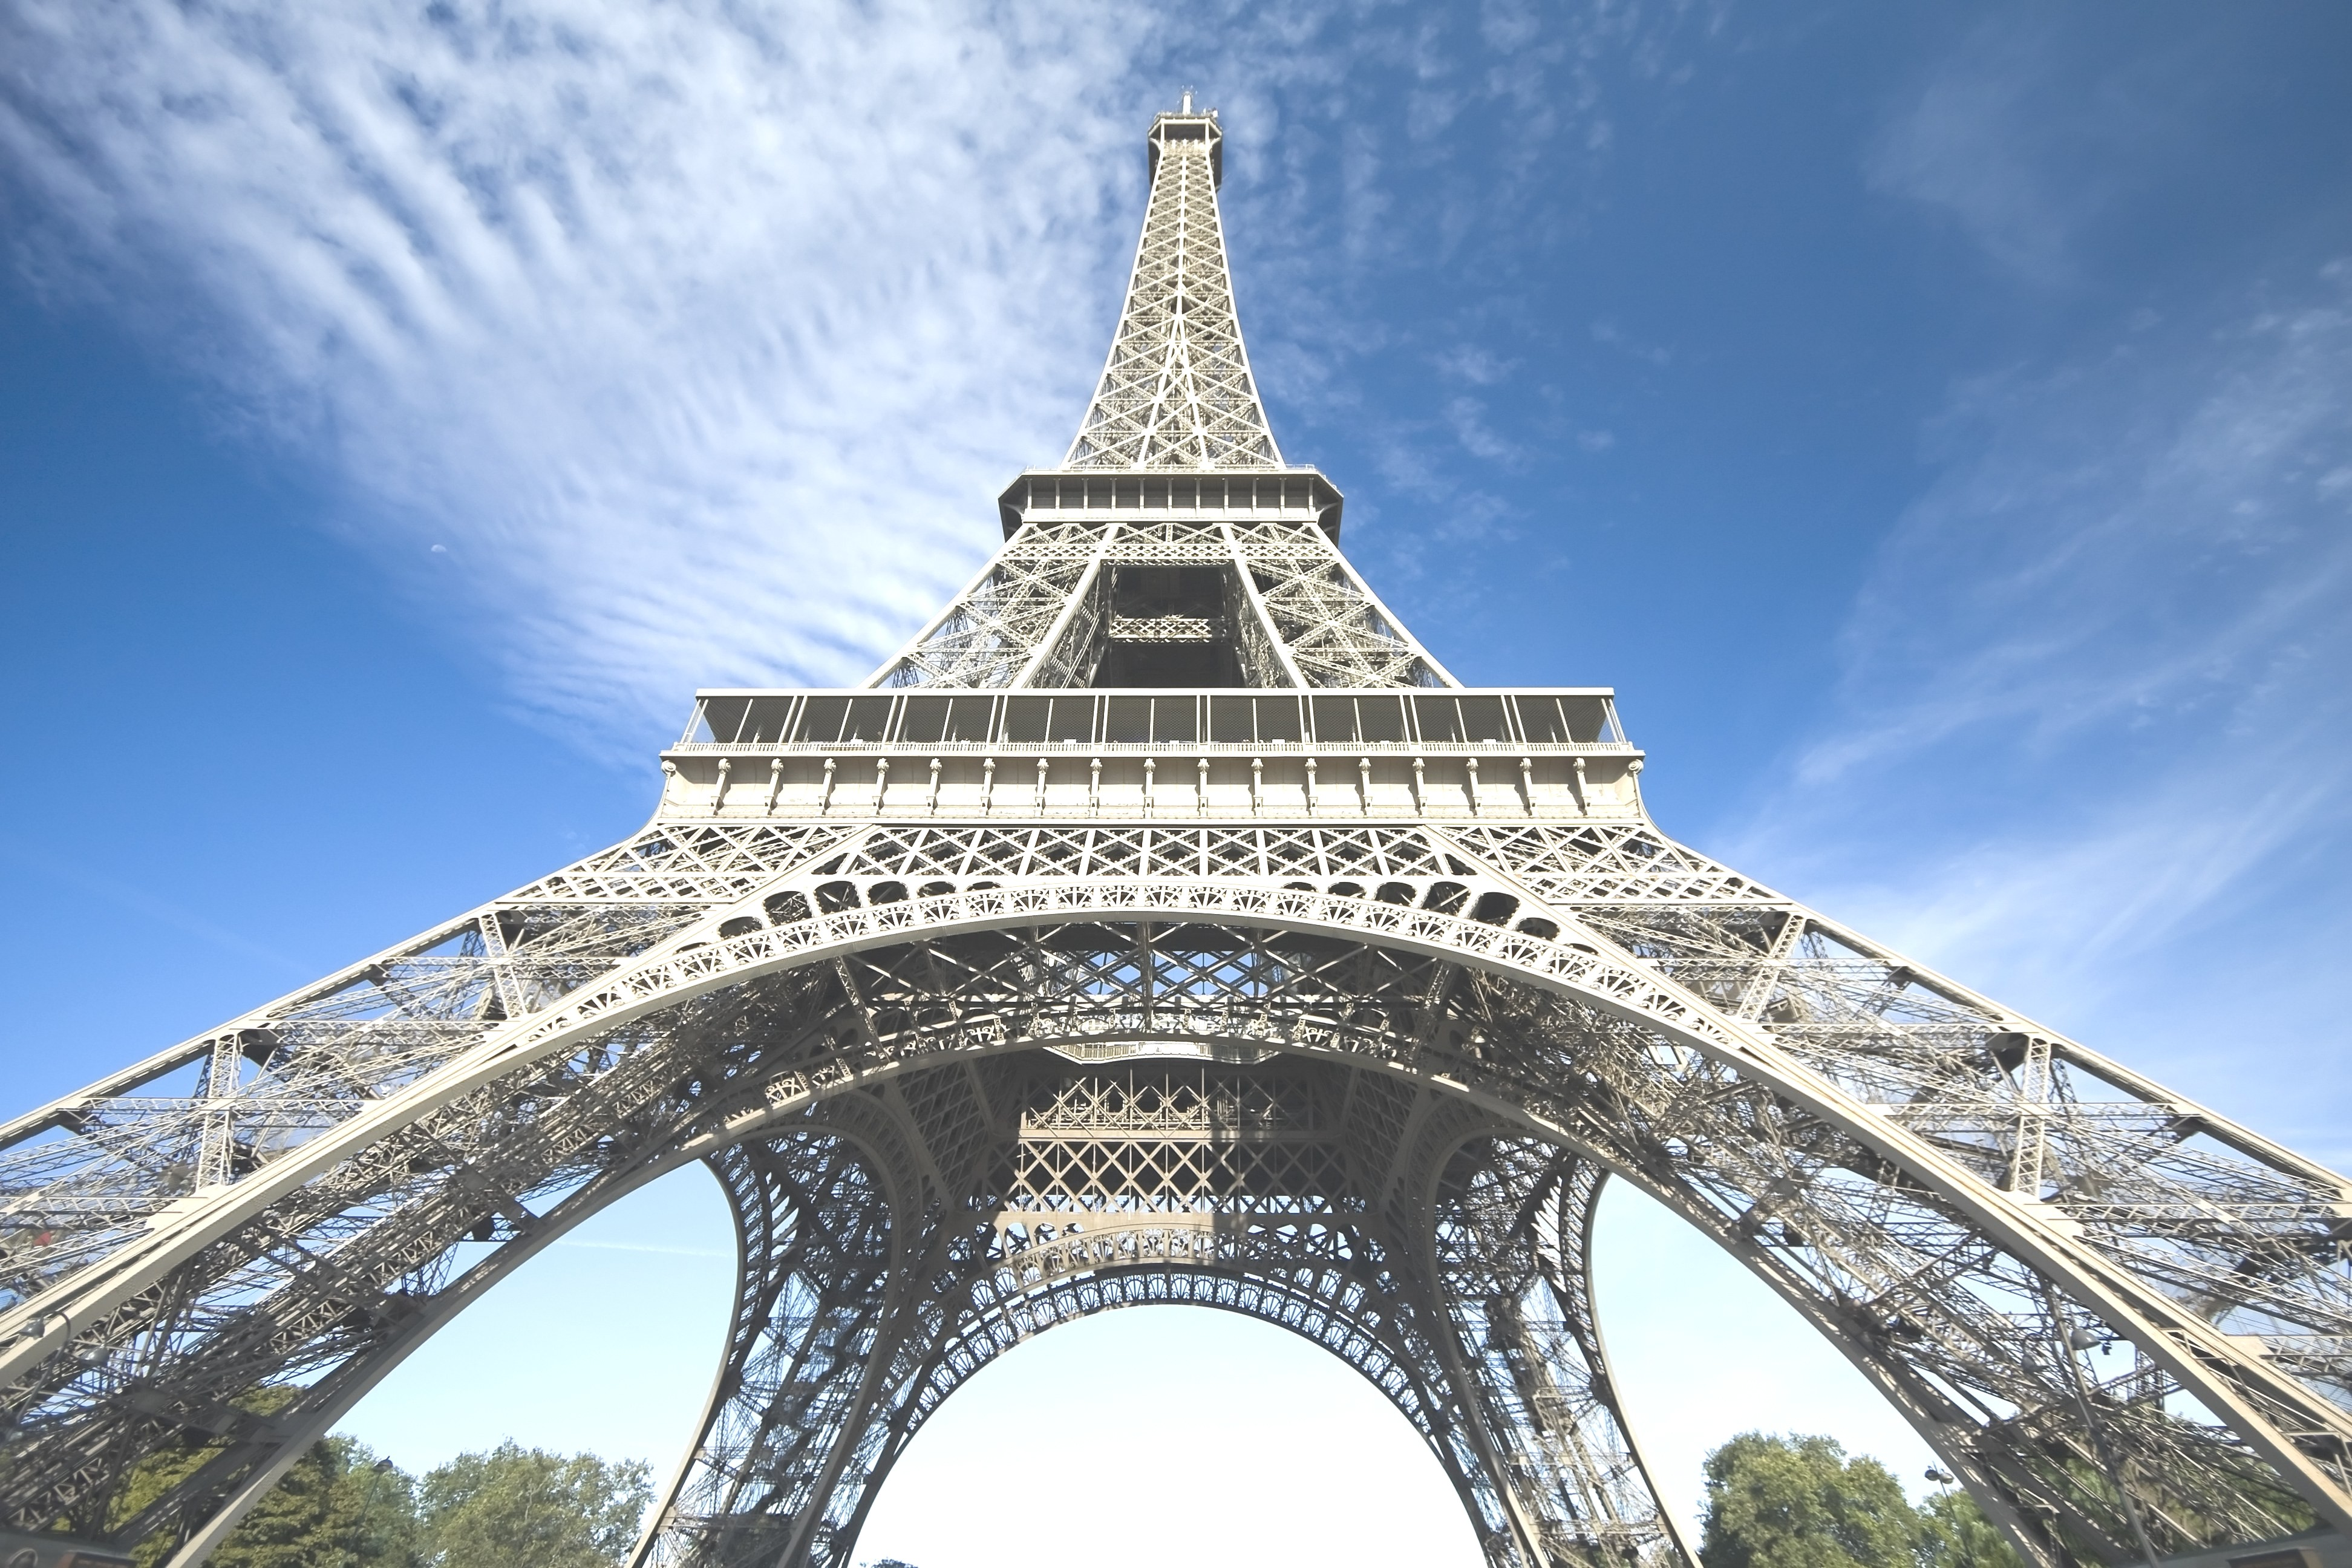
\includegraphics[width=\linewidth]{./img/6b.jpg}
    \caption{Brightness +50}
  \end{subfigure}
\end{figure}

\subsection*{3. Blending images}

The task get the blending ratio from users, and then compute the average pixel's colors between two images by the ratio.
\\\\
Here is the image blended between Effeil image and national flag of France, with ratio = 0.5.

\begin{figure}[H]
  \centering
  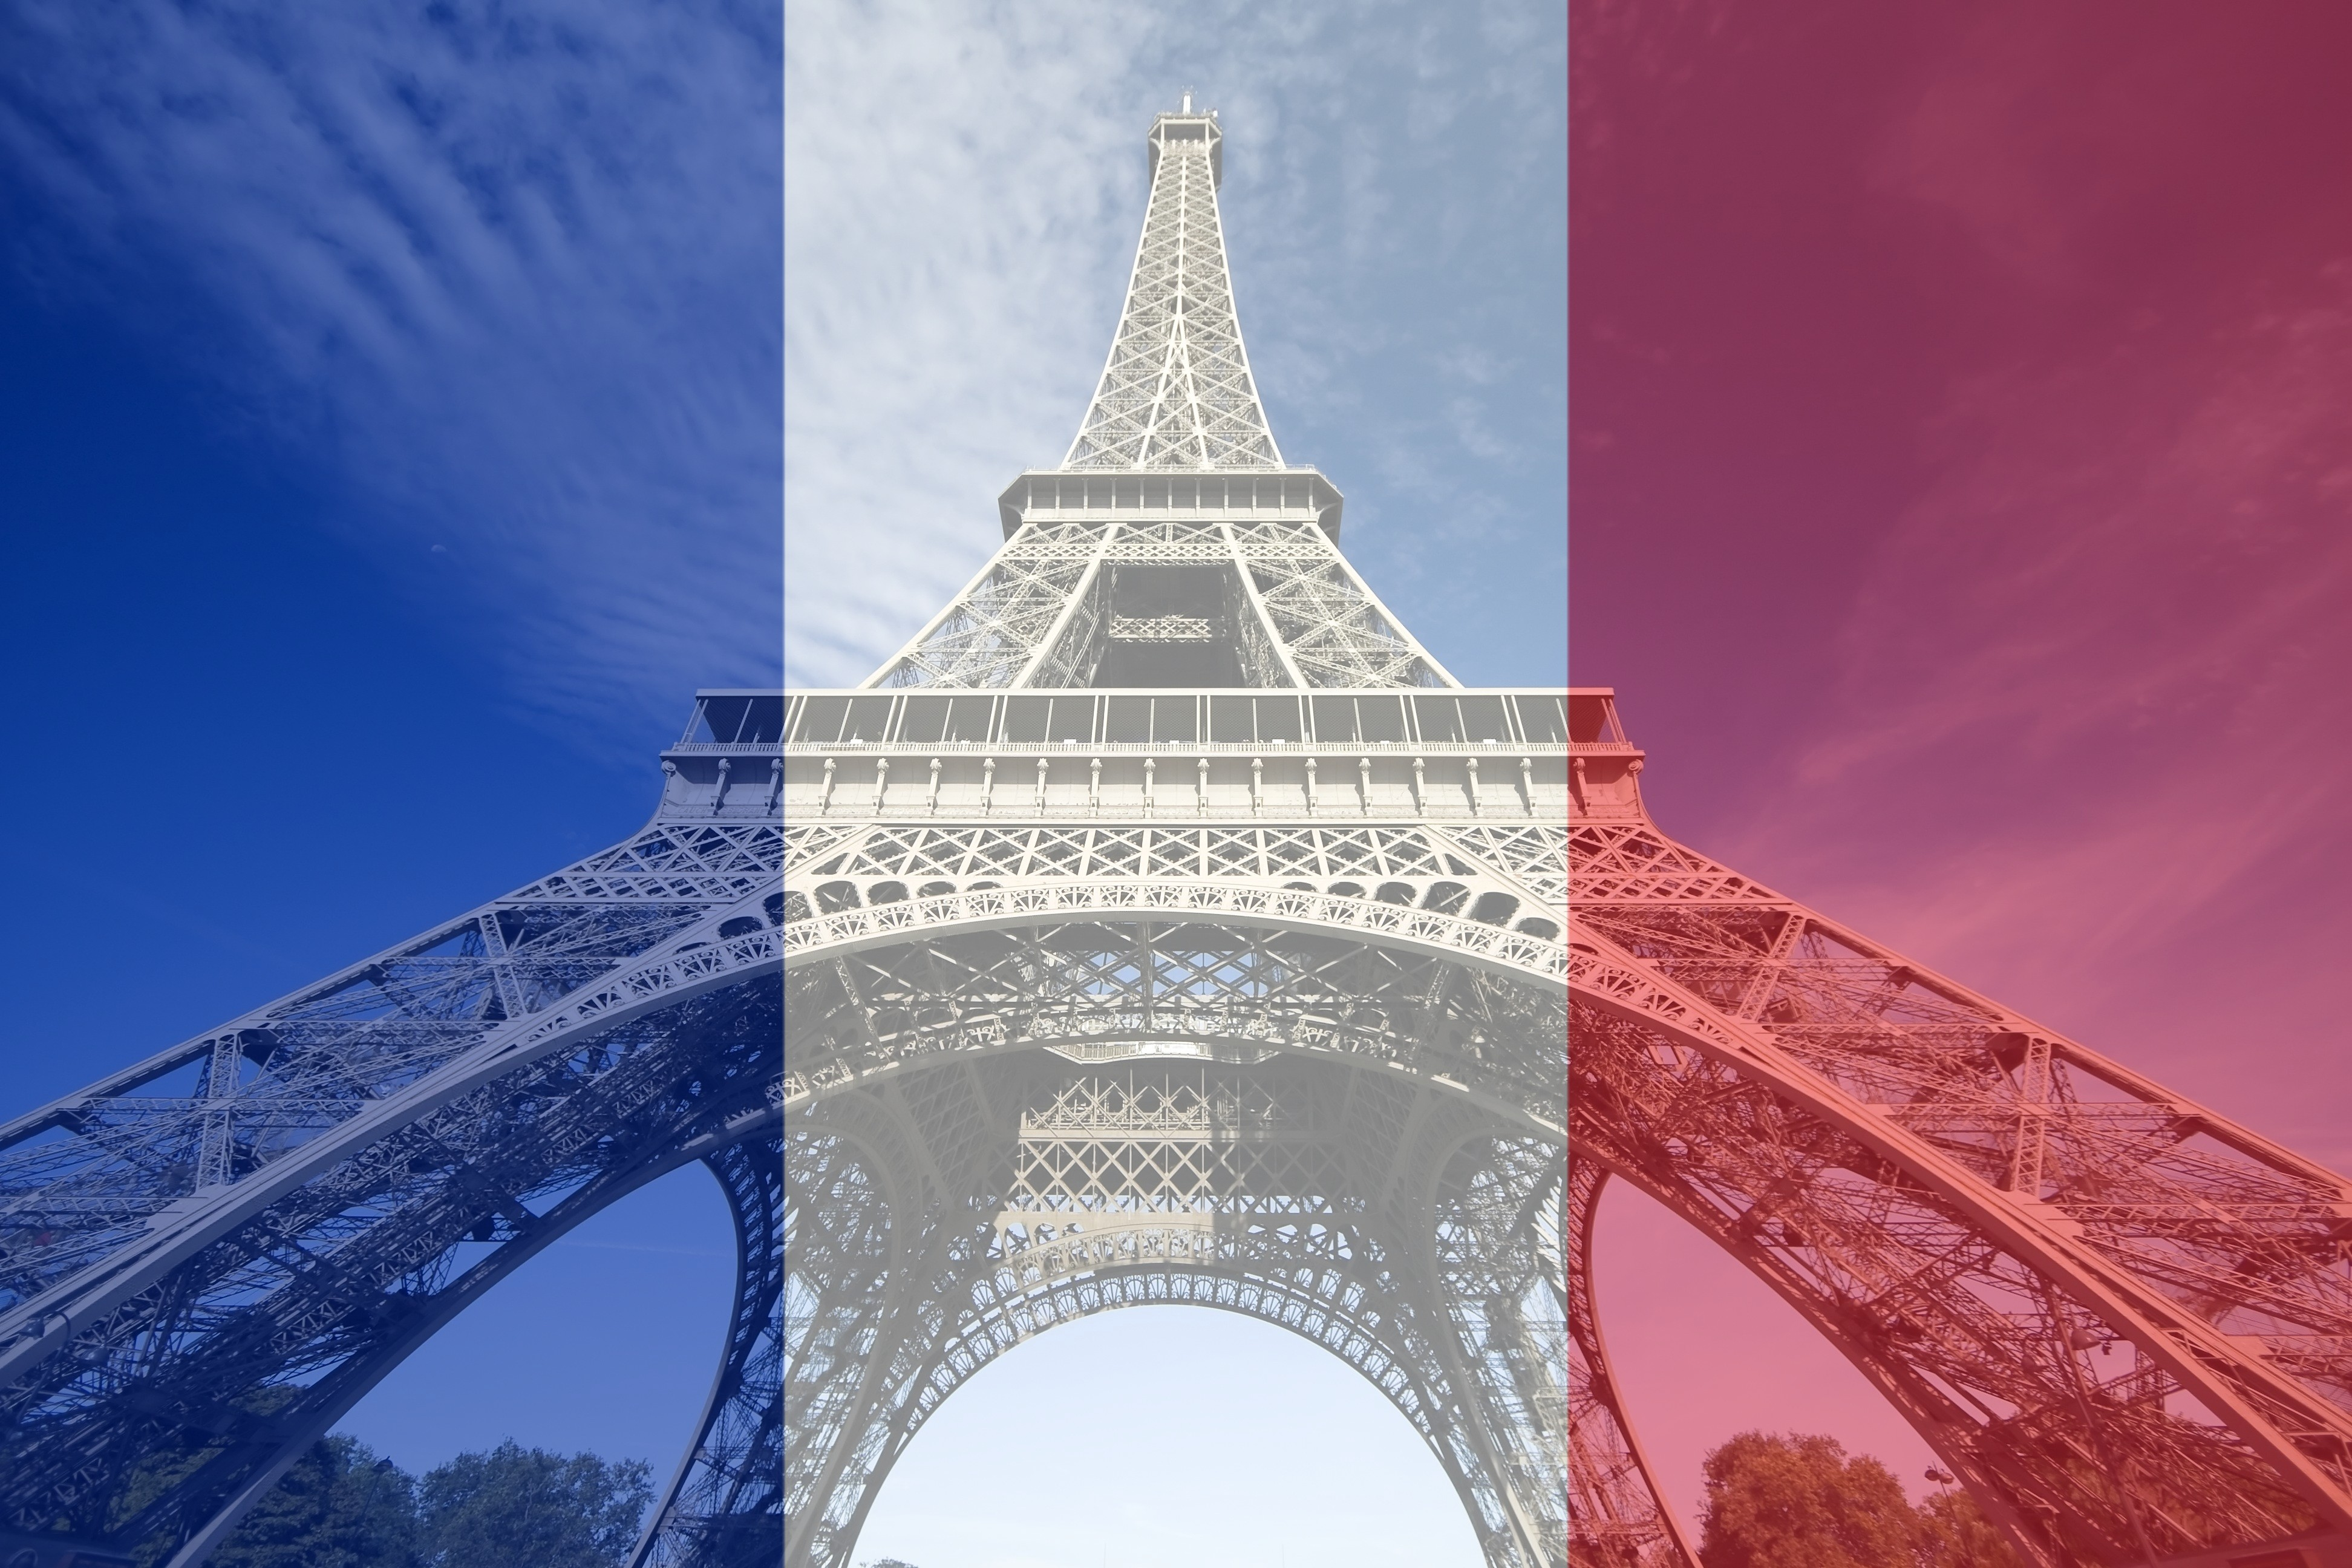
\includegraphics[width=0.7\linewidth]{./img/6c.jpg}
\end{figure}

\end{document}
